%%========================================================================
%% LaTeX scriptiesjabloon
%%========================================================================


%%========================================================================
%% Preamble
%%========================================================================

\documentclass[pdftex,a4paper,12pt,twoside]{report}

%%---------- Extra functionaliteit ---------------------------------------
\usepackage{tipa}								% phonetics
\usepackage[utf8]{inputenc}						% Accenten gebruiken in tekst (vb. é ipv \'e)
\usepackage{amsthm}								% Theorum package
\usepackage{amsfonts}        					% AMS math packages: extra wiskundige
\usepackage{amsmath}         					% symbolen (o.a. getallen-
\usepackage{amssymb}         					% verzamelingen N, R, Z, Q, etc.)
\usepackage[UKenglish]{babel}					% Taalinstellingen: woordsplitsingen,
                             					% commando's voor speciale karakters
                             					% ("dutch" voor NL)
							 					% ("UKenglish" voor brits engels)
\usepackage{eurosym}         					% Euro-symbool €
\usepackage{graphicx}        					% Invoegen van tekeningen
\usepackage[pdftex,bookmarks=true]{hyperref}	% PDF krijgt klikbare links &  verwijzingen, inhoudstafel
\usepackage{listings}        					% Broncode mooi opmaken
\usepackage{multirow}        					% Tekst over verschillende cellen in tabellen
\usepackage{rotating}       	 				% Tabellen en figuren roteren
\usepackage{natbib}          					% Betere bibliografiestijlen
\usepackage{fancyhdr}        					% Pagina-opmaak met hoofd- en voettekst
\usepackage{graphicx}		 					% Om figuren te kunnen verwerken
\usepackage[small,bf,hang]{caption}				% Om de captions wat te verbeteren
\usepackage{subcaption}		 					% subcaptions
% \usepackage[nottoc]{tocbibind}					% Bibliografie en inhoudsopgave in ToC; zie tocbibind.dvi
%%---------- Layout ------------------------------------------------------

% hoofdingen, enz.
\pagestyle{fancy}

%voorkom overlap van sectie titels en chapter titel
\renewcommand{\sectionmark}[1]{} 

% lijn, wordt gebruikt in titelpagina
\newcommand{\HRule}{\rule{\linewidth}{0.5mm}}

% Leeg blad
\newcommand{\emptypage}{
\newpage
\thispagestyle{empty}
\mbox{}
\newpage
}
 
% Gebruik een schreefloos lettertype ipv het "oubollig" uitziende
% Computer Modern
\renewcommand{\familydefault}{\sfdefault}     

% Commando voor invoegen Java-broncodebestanden (dank aan Niels Corneille)
% Gebruik: \codefragment{source/MijnKlasse.java}{Uitleg bij de code}
\newcommand{\codefragment}[2]{ \lstset{%
  language=java,
  breaklines=true,
  float=th,
  caption={#2},
  basicstyle=\scriptsize,
  frame=single
}
\lstinputlisting{#1}}

% Theorum definitions and style
\theoremstyle{plain} \newtheorem{theorem}{Theorem} \newtheorem{proposition}{Proposition} \newtheorem{lemma}{Lemma} \newtheorem*{corollary}{Corollary}

\theoremstyle{definition} \newtheorem{definition}{Definition} \newtheorem{conjecture}{Conjecture} \newtheorem*{example}{Example} \newtheorem{algorithm}{Algorithm}

\theoremstyle{remark} \newtheorem*{remark}{Remark} \newtheorem*{note}{Note} \newtheorem{case}{Case}

%%---------- Custom Commands ---------------------------------------
% CAPTCHA
\newcommand{\captchasp}{CAPTCHA }
\newcommand{\captcha}{CAPTCHA}

%%---------- Documenteigenschappen ---------------------------------------
%% Vul dit aan met je eigen info:

% Je eigen naam
\newcommand{\studenta}{Pieter {Van Eeckhout}}

% Eventueel naam van een medestudent.
% Laat in commentaar indien niet van toepassing
%\newcommand{\studentb}{Steven Stevens}

% De naam van je stage-/bachelorproefbegeleider
\newcommand{\begeleider}{Johan {Van Schoor}} 

% De naam (én firma/organisatie) van je mentor/promotor
% Laat in commentaar indien niet van toepassing
%\newcommand{\mentor}{Jan Janssen, ACME Inc.}

% De titel van je scriptie/stageverslag
\newcommand{\titel}{Solving \captchasp using neural networks}

% Ondertitel
\newcommand{\ondertitel}{}

% Datum van indienen
\newcommand{\datum}{10 June 2013}

% Academiejaar
\newcommand{\academiejaar}{2012-2013}


%%========================================================================
%% Inhoud document
%%========================================================================

\begin{document}

%%---------- Front matter ------------------------------------------------
%% Het voorblad - Hier moet je in principe niets wijzigen.

\begin{titlepage}
\begin{center}

\includegraphics[width=4cm]{./img/FBO-EN.png}\\[.5cm]




Professional Bachelor in Applied Computer Science\\
Academic year \academiejaar

\vfill

\HRule \\[0.4cm]
{ \huge \bfseries \titel}\\[0.4cm]
\HRule \\[0.4cm]

{\Large \ondertitel}\\[0.4cm]

Submitted on \datum

\vfill

% Studenten en begeleiders
\begin{minipage}{0.49\textwidth}
\begin{flushleft}
\emph{Student\ifdefined\studentb en\fi :}\\
\studenta \\
\ifdefined\studentb \studentb \fi\par
\end{flushleft}
\end{minipage}
\begin{minipage}{0.49\textwidth}
\begin{flushright}
\emph{Mentor:}\\ \begeleider\\
\ifdefined\mentor \emph{Mentor:}\\ \mentor \fi
\end{flushright}
\end{minipage}

\end{center}

\end{titlepage}

% Schutblad

\emptypage

% Herhaling titelblad

\begin{titlepage}
\begin{center}
HoGent Business \& Information Management\\
Professional Bachelor in Applied Computer Science\\
Academic year \academiejaar

\vfill

\HRule \\[0.4cm]
{ \huge \bfseries \titel}\\[0.4cm]
\HRule \\[0.4cm]

{\Large \ondertitel}\\[0.4cm]

Submitted on \datum

\vfill

% Studenten en begeleiders
\begin{minipage}{0.49\textwidth}
\begin{flushleft}
\emph{Student\ifdefined\studentb en\fi :}\\
\studenta \\
\ifdefined\studentb \studentb \fi\par
\end{flushleft}
\end{minipage}
\begin{minipage}{0.49\textwidth}
\begin{flushright}
\emph{Mentor:}\\ \begeleider\\
\ifdefined\mentor \emph{Mentor:}\\ \mentor \fi
\end{flushright}
\end{minipage}

\end{center}

\end{titlepage}

%% Inhoudstafel

\tableofcontents


%%---------- Kern --------------------------------------------------------

\begin{abstract}

%% De "abstract" of samenvatting is een kernachtige (max 1 blz. voor een
% thesis) synthese van het document. In ons geval beschrijf je kort de
% probleemstelling en de context, de onderzoeksvragen, de aanpak en de
% resultaten. 

%TODO
TODO
\end{abstract}

\chapter*{Preamble}
\label{ch:preamble}
First, dear reader, I would like to thank you for taking the time to read this thesis. Without an audience this entire endeavour would not mean as much as it does right now, while you are reading its results. I personally believe this is because I would like my life not to go unnoticed. So if this thesis helps, or influences you in any way, then this work has gained more meaning.\\Second I would like to thank the following people who have made it possible for me to arrive at this point. Special thanks and mentions go to:
\begin{itemize}
\item my parents, for supporting me and giving me the opportunity and supplying the means for me to pursue my academic career.
\item my girlfriend, Anne Charlotte Magdaraog Mendoza. Because she has helped me countless times through the rough spots. Not once did she complain about the time consuming job of writing this work.
\item my good friends, willing proof readers and content critics: Wouter Dekens, Patrick Van Brussel and Thijs van der Burgt.
\item Johan Van Schoor and Bert Van Vreckem for the support, organisation, guidance and feedback.
\end{itemize}
Bare in mind that this is not an exclusive list. Finally I would like to thank all the other people who are not mentioned by name: such as the teaching and support staff at University College Ghent.\\\\Ghent BELGIUM, June 2013
\begin{center}
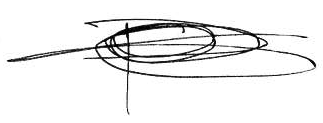
\includegraphics[width=5cm]{./img/signature.png}\\[.5cm]
\studenta
\end{center}
\chapter{\titel}
\label{ch:introduction}
\paragraph{The target audience.}
This thesis was written with an audience in mind that already has some technical understanding of computers and how they operate on hardware level (processor etc.). If you feel that your current knowledge is insufficient, or just want to read up some more, then I refer you to the ''How Computers Work - Processor and Main Memory'' \citep{Young2001} e-book.
\paragraph{The history of SPAM.} 
Ever since the internet found its way into our daily life, there have been people out there who don't always have other people's best interest in mind. I am referring to spammers, people aiming to advertise their product, services, etc \ldots in an aggressive manner. The methods of advertising include but are not limited to: \begin{itemize}
\item Sending bulk emails without the recipients permission (SPAM). 
\item Posting irrelevant links and information on fora and various social media.
\item Flooding chat channels with their links and information. 
\end{itemize}
These emails, posts and messages inconvenience the end-users, requiring time to filter out the junk. The economic costs of SPAM has led to a decrease in the Japanese GDP by 500 billion Yen (3.78 billion Euro) in 2004 and were projected to reach a decrease of 1\% of the total GDP by 2010 unless adequate countermeasures were taken \citep{Ukai2007}. \citep{Khong2004} researched the economic arguments for regulating junk mails and the efficiency of these regulations.
\paragraph{Birth of CAPTCHA.} 
The two previously mentioned researches signify the importance and impact of SPAM on our daily life. The users of the internet quickly tried to implement methods to prevent spammers from spreading their advertisements to the masses. Several prevention and detection methods and systems were developed successfully. These methods and mechanisms range from hidden text to invalid HTML tags, all used to confuse and interrupt automated programs. One of the methods developed to prevent SPAM is a CAPTCHA test. CAPTCHA is an acronym based on the word ''capture'' and stands for 'Completely Automated Public Turing test to tell Computers and Humans Apart'. An attempt to trademark  the term was made by Carnegie Mellon University on 15 October 2004, but the application was eventually dropped on 12 April 2008
\paragraph{Spammers fight back.}
All these prevention and detection methods did not stop the spammers from trying to reach an audience as large  as possible. The spammers rely on a large target audience because of the return rates being as low as 0.0023\% \citep{Cobb2003}. The spammers started to device ways to circumvent or break the existing systems in order to reach a large enough audience. One of these methods is solving CAPTCHA tests by making use of the adaptive learning and pattern recognizing capabilities of neural networks. These networks can be used to recognize letters from images with adversarial clutter.
This is the area I will focus on in this thesis. This thesis will list some of the difficulties regarding the extraction of relevant data from a CAPTCHA and how to possibly overcome these difficulties. However the main focus will be on understanding the inner workings of neural networks and on searching for the types and configuration of neural networks best used for pattern recognition.
\chapter{Premise and research questions}
\label{ch:Premise}
\section{Premise}
\label{sec:Premise}
The main objective of this thesis is to ascertain whether neural networks are capable of solving the current generation of CAPTCHA images. we will define the premise  as following:\\\\
\emph{''Are neural networks a viable tool for solving the current generation of CAPTCHA?''}
\section{Research questions}
\label{sec:researquestions}
The research can be divided into two separate subjects. If one was to develop software for automatic CAPTCHA solving, the following questions and problems would need to be addressed.
\paragraph{\captcha :}
\begin{itemize}
\item What are the different types of CAPTCHA?
\item How can the distorted text be extracted?
\end{itemize}
\paragraph{Neural networks:}
\begin{itemize}
\item How do neural networks operate?
\item Which types of neural networks are well suited for pattern recognition?
\item What network configuration would perform best?
\end{itemize}
\paragraph{General:}
\begin{itemize}
\item How future proof would this solution be?
\item Is there enough economic incentive to invest in development?
\end{itemize}
\chapter{Methodology}
\label{ch:methodology}
\paragraph{Research philosophy.}
%TODO
TODO
\paragraph{Research approach.}
%TODO
TODO
\paragraph{Data Analysis.}
%TODO
TODO
\chapter{Corpus}
\label{ch:corpus}
\section{CAPTCHA}
\label{sec:captcha}
\subsection{CAPTCHA, an explanation}
A CAPTCHA (pronounced \textipa{/'\phonetic{k\ae p.\textteshlig \textschwa /}}) is a type of challenge-response test that aims to make sure the response was made by a human. These tests are designed in such a manner that they should be easy to generate and grade by a computer, and at the same time be difficult for a computer to solve. Yet a human should be able to solve the test without much difficulty. If a test was solved successfully one can assume that the response was entered by a human.\\These test are mostly found on sites where one would like to prevent the access to unwanted bots. This is because having lots of spam on a site or in a service can have real detrimental consequences for that site or service. This is because most contemporary interactive sites store and serve their content from a database. When a database gets filled up the site can become slow and sluggish, reducing the customer's experience. This is only one of the many useful applications of CAPTCHAs. On the other hand, legitimate users also need to solve these tests, so it requires them to perform an extra task before they can post their content, create an email or view a certain page. While this 'simple' extra task does not seem like a large barrier, it does inconvenience some people enough to prevent them from posting valid content. This problem becomes even more apparent when dealing with non-native speakers \citep{Banday2011}. Protecting your site with a CAPTCHA can even have a detrimental effect on the conversion rates\footnote{\url{http://www.seomoz.org/blog/captchas-affect-on-conversion-rates}}.
\subsection{The history of CAPTCHA}
Moni Naor was the first one to think of the concept of CAPTCHA in 1996. He proposed that reverse Turing testing, as CAPTCHAs are often called, should consist of ''tasks where humans excel in performing, but machines have a hard-time competing with the performance of a three year old child.'' Some of these tasks were \citep{Naor1996}:
\begin{itemize}
\item gender recognition
\item understanding facial expressions
\item understanding handwriting
\item filling in words
\end{itemize}
In 1997 'Yahoo!' was having a gargantuan problem with spammers using bots to create free email addresses used to spread a huge amount of unwanted advertisement, giving Yahoo email adresses a bad reputation. 'Yahoo!' contacted Carnegie Mellon University\footnote{\url{http://www.cylab.cmu.edu/research/projects/2008/captcha-project.html}} for help, by 2000 the first real CAPTCHA as we know them was invented \citep{Egen2009}. These were also the people who first used the term ''CAPTCHA'' and tried to trademark it.\\As computing power increased, so did the amount of CAPTCHA tests being broken. By 2008 there was an 30\% to 60\% success rate on the most used CAPTCHA systems \citep{Yan2008}. As a  response to this Von Ahn and his team at Carnegie Mellon University released reCAPTCHA (Figure ~\ref{fig:reCAPTCHA}, page ~\pageref{fig:reCAPTCHA}) in September 2008, a popular system which is still in use.\\CAPTCHAs have always undergone changes once it became clear a certain generation method didn't stop the spammers any more. The first CAPTCHAs generated by EZ-Gimpy for 'Yahoo!' looked completely different from the CAPTCHAs that are currently being generated. A good example of the adaptive nature of CAPTCHAs is reCAPTCHA, were you can see the changes depending on when a CAPTCHA was generated. (Figure ~\ref{fig:captchaEvolution}, page ~\pageref{fig:captchaEvolution})
\subsection{Types of CAPTCHA}
Following is a list and description of the different types of CAPTCHA, courtesy of \citep{Sauer2008}.
\begin{description}
\item[Character based]In this category a string of characters is presented to the user. This string can contain either words or random alphanumeric characters. The task is to identify the string of characters.
\item[Image based]In this category images or pictures are presented to the user. This is normally in the form of an identifiable real-world object, but can also be presented in the form of shapes. The task is to identify the object shown in the picture.
\item[Anomaly based]In this category a series of different objects, shapes, characters,\ldots is presented to the user. The task is to determine which object, character or shape does not belong in a set of images displayed on the screen.
\item[Recognition based]In this category all previous categories can be used. The user is tasked to determine what is being presented to them and respond accordingly.
\item[Sound based]In this category an audio version of a CAPTCHA is presented. The task is to identify the words and letters or image presented to the user.
\end{description}
\subsection{Data extraction}
As previously stated, the data extraction part of solving CAPTCHAs is not the main focus of this thesis. Therefore I will not give in-depth explanations of the algorithms used and described here.\\\\CAPTCHAs are by design tough to solve for a computer. The majority of times a CAPTCHA gets cluttered with noise, or the letters get crowed together. This crowding or noise makes it so that the characters on the image are not separate entities. This is to impede the segmentation of the CAPTCHA. Measures against segmentation are necessary to prevent an OCR\footnote{Optical Character Recognition} algorithm from simply reading and solving the test. This could be possible, as computers can (given the right algorithms) be very efficient at pattern recognition. People trying to solve the CAPTCHA test automatically, have to separate the individual characters first before they can pass the characters to an OCR algorithm for classification.\\\citep{Yan2008} described a working segmentation algorithm in 2008, but \citep{Huang2010} has significantly improved on the performance, so it should be able to segment the contemporary CAPTCHAs.\\In the unlikely case that the CAPTCHAs you are trying to solve don't have the segmentation issues, then you can first try to reduce the noise and then segment the characters by using the flood-fill method, as described by \citep{Cai2008}.
\subsection{The future of CAPTCHA}
\begin{figure}
	\centering
	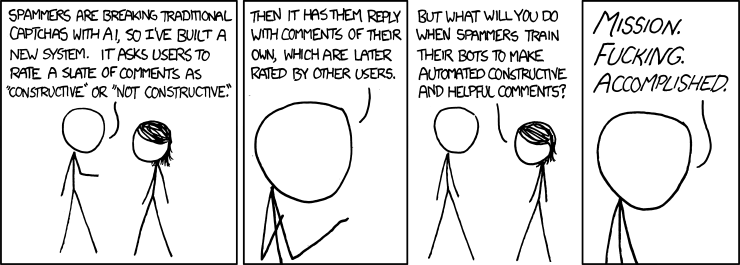
\includegraphics[width=13.75cm]{./img/xkcd-captcha-evolution.png}
	\caption{xkcd on the future of CAPTCHA (Source: \url{http://www.xkcd.com/810/}, accessed on 2013/05/28)}
	\label{fig:xkcdCAPTCHA}
\end{figure}
The arms race between the makers of CAPTCHA systems and people trying to break them favoured the defender. This is different from other computer security arms races, where the odds are in favour of the adversary. This is because CAPTCHA has broken the traditional pattern where the attacker's role is to generate new instances while the defender must recognize them, recognizing a problem is almost always harder than generating them. Websites and services using CAPTCHA can easily change the CAPTCHA generation algorithm, creating new unsolvable CAPTCHAs, while the attackers now have the challenging recognition problem. This battle has brought advances to the field of Automated Pattern Recognition and Artificial Intelligence. Some people even believe that eventually the solving algorithms will become so sophisticated they could be classified as a sentient AI\footnote{\url{http://thenextweb.com/2009/10/15/inevitable-future-captcha/}} (Figure~\ref{fig:xkcdCAPTCHA}).\\
All the positive aspects and technological innovations aside, CAPTCHAs are inherently flawed. As the solving agents got better, the CAPTCHAs became harder. We have reached the point where the average user is having difficulties solving the standard CAPTCHAs\footnote{\url{http://www.internetevolution.com/author.asp?section_id=587&doc_id=259406}}. \\\\
CAPTCHA of the future will need to explore completely new test systems. As an example of this, \citep{Sauer2008} and colleges did a small research about how the current CAPTCHA (even the audio CAPTCHA) has serious shortcomings when trying to accommodate for blind or visually impaired users. They suggest a new system were the sound and image part of the test are integrated, opposed to the current system where the audio part and the visual part are on independent development and maintenance paths. With their suggested test all visually impaired and hearing impaired users should be able to solve the test.\\\\
But even the newly developed systems will eventually succumb to the ever increasing computing power. The question is whether CAPTCHAs are the right way to prevent spammers, because how many ''unsolvable CAPTCHA'' (Figure ~\ref{fig:ImpossibleCaptcha}, page ~\pageref{fig:ImpossibleCaptcha}) is a user going to tolerate before giving up? The malcontent of some has even led to the creation of intentionally unsolvable CAPTCHAs (Figure ~\ref{fig:CRAPCHA}, page ~\pageref{fig:CRAPCHA}) through a service called ''CRAPCHA''\footnote{\url{http://crapcha.com/}}, aimed at ridiculing the real CAPTCHA services.
\begin{quote}
It would seem evident from years of use and research that CAPTCHAs are far from perfect as a solution. Remove spammers from the equation and we remove the need for CAPTCHAs entirely; this is the mentality we should be aiming for. The perfect CAPTCHA is no CAPTCHA at all. \citep{Bushell2011}
\end{quote}\newpage
\section{Neural Networks}
\label{sec:neuralnetworks}
The following section is a synthesis of 2 books describing neural networks, so similarities in structure and wording will be found. However, no malicious copyright infringement is intended. The two books used are ''Neural Networks'' by David Kriesel \citep{Kriesel2013} and ''Introduction to neural networks with Java'' by Jeff Heaton \citep{Heaton2005}.
\subsection{The concept of time}
When we describe time in the context of neural networks, we denominate the number of cycles of the neural network. In this context time is split into discrete steps.
\begin{definition}(The Concept of time). We reference the current time as $(t)$ the next step in time is referred to as $(t+1)$ and the previous step as $(t-1)$. The other steps further ahead or behind are referenced analogously. \end{definition} When we refer to a certain point in time for mathematical variables (e.g. $net_j or o_i$) we will do this as following $net_j(t-1) or o_i(t+3)$.
\subsection{The components of an artificial neural network}
An artificial neural network is made up by basic processing units, the \emph{neurons}, and directed weighted connections between these neurons. The strength of the connection is called the weight, this is expressed as $w_{i,j}$ for the connection between neuron $i$ and neuron $j$
\begin{definition}
(Neural network). A neural network is a sorted triple $(N, V, w)$ which contains two sets $N, V$ and a function $w$. $N$ is a set of neurons, $V$ is a set of connections where for each connections between neuron $i$ and $j$ applies $\{(i,j)|i,j \in  \mathbb{N}\}$, $w$ is a function ($w : V \to \mathbb{R}$) defining the weights. Where $w((i,j))$ defines the weight for the connection between neuron $i$ and neuron $j$, shortened to $w_{i,j}$.
\end{definition} Depending on the implementation, a connection int the network does not exist or has no influence when the weight is undefined or equal to zero. The weight can be combined in a square \emph{weight matrix} $W$, or in a \emph{weight vector} $W$. The row number indicates where a connection begins and the column number where it ends. In this representation, a zero indicates a non-existing or inactive connection. This kind of representation is also called a \emph{Hinton Diagram} (Figure ~\ref{fig:HintonDiagram}, page ~\pageref{fig:HintonDiagram}).
\subsubsection{Neuron Data Processing}
Upon closer inspection, we can see that the neuron and its connections are made up out of several other distinguishable components and processes. which we will discuss more in-depth in the following sections.
\begin{figure}
\centering
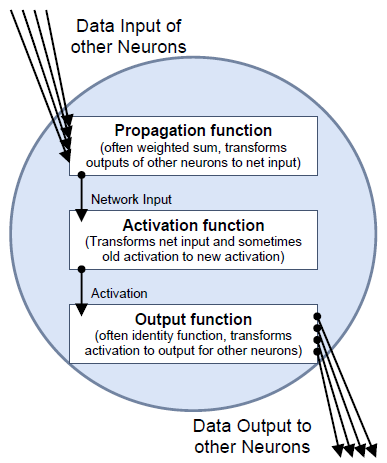
\includegraphics[width=7cm]{./img/Neuron_Dataprocessing.png}
\caption{Neuron Data processing (Source: \citep{Kriesel2013} page 39, Figure 3.1)}
\end{figure}
\subsubsection{Propagation function}
In a network there will likely be more then one neuron linking to neuron $j$. Which means that each neuron one of these neurons will pass its output to neuron $j$. The propagation function receives all these outputs $o_{i_{1}},\dotsc,o_{i_{n}}$ of the neurons $i_1,i_2,\dotsc,i_n$ and combines those into a single value, the \emph{network input} $net_j$, based on the connection weights $w_{i,j}$.
\begin{definition}
(Propagation function and network input) The network input, or $net_j$, can be calculated with the propagation function $f _{prop}$ as follows:
\begin{equation}
net_j = f _{prop}(o_{i_{1}},\dotsc,o_{i_{n}},w_{i_{1},j},w_{i_{n},j})
\end{equation}
Where $I = \{i_1,i_2,\dotsc,i_n\}$ is the set of neurons so that $\forall z \in \{1,\dotsc,n\} : \exists w_{i_{z},j}$. The \emph{weighted sum} is a very popular, and the most used propagation function.
\begin{equation}
net_j = \sum_{i \in I}(o_i \cdot w_{i,j})
\end{equation}
\end{definition}
\subsubsection{Neuron threshold value}
\begin{definition}
(Threshold value in general). The threshold value $\Theta_j$ for neuron $j$ is uniquely assigned to $j$ and defines the position of the maximum gradient of its activation function.
\end{definition}
This means that the activation function of a neuron will react very sensitive to changes when $net_j$ is around the threshold value. 
\subsubsection{Neuron activation function.}
\paragraph{Activation status.}Neurons can change in activation status. A neuron's activations state depends on the $net_j$, the previous activation state and the activation function. A neurons activation state is important, because this will influence a neuron's reaction to the $net_j$.
\paragraph{Activation function.}
The activation, also called the transfer function, $a_j$ of neuron $j$ depends on on previous states, so this will change overtime. The activation function uses the network input $net_j$, the threshold value and the previous activation state $a_j(t-1)$ to create a new \emph{activation state}. The neuron activation function is also called the identity.
\begin{definition}
(activation and activation function). In neuron $j$ the activation function can be described as
\begin{equation}
a_j(t) = f _{act}(net_j(t),a_j(t-1),\Theta_j)
\end{equation}
\end{definition}
\subparagraph{Binary threshold function.}
the binary threshold function, also called the \emph{Heaviside function}, is the simplest activation function as can only take on two values. The activation will change, depending on whether the input value is above or below the threshold value. In either case the function changes from one value to another. This activation function doesn't have a variable, hence it's derivative is 0. This makes back-propagation learning impossible 
\subparagraph{Fermi function.}
The Fermi function, also called the logistic function, uses following equation. from the equation we can derive that the Fermi function maps a range of values between $(0,1)$. It's function is describe as following:
\begin{equation}
\displaystyle \frac{1}{1+e^{-x}}
\end{equation}
\subparagraph{hyperbolic tangent.}
The hyperbolic tangent function maps to values within the range of $(-1,-)$. It's function is describe as following:
\begin{equation}
\tan(x)
\end{equation}
\subparagraph{Fermi function with temperature parameter.}
The Fermi function can be expanded by adding a temperature parameter. The smaller this parameter becomes the colder the activation function becomes, the steeper the gradient of the activation function becomes. And visa versa. By making the temperature parameter very small, we can emulate the Heaviside activation function's behaviour. The extended Fermi activation is described as following:
\begin{equation}
\displaystyle \frac{1}{1+e^{\frac{-x}{T}}}
\end{equation}
\subsubsection{The bias neuron}
\label{subsubsec:biasneuron}
The bias neuron (also called the on neuron) is a technical trick. the purpose of a bias neuron is to represent a neurons threshold value as a connection weight. As said before the activation of a neuron depends on its threshold value, however theses threshold values are stored inside the neuron itself. This makes it complicated to access and use in the activation function, or to train the threshold value. This is where the bias neuron comes in.\\\\Threshold values $\Theta_{j_{i}}, \dotsc ,\Theta_{j_{n}}$ for neurons $j_1,j_2, \dotsc ,j_n$ can be expressed as a connection weight of a constantly firing neuron. This constantly firing neuron is the bias neuron. To implement this change, an additional neuron, whose output is always 1, will be added tot the network and connected to neurons $j_1,j_2, \dotsc ,j_n$. The newly made connections' weights will be set to the negative threshold values. $w_{BIAS,j_{n}} = - \Theta_{j_{n}}$\\\\Now that the threshold values are implemented as connection weight, the threshold value $\Theta_{j_{n}}$ of neurons $j_1,j_2, \dotsc ,j_n$ is then set to 0. This also means that the threshold value can be directly trained together with the connection weight. This makes the learning process considerably easier. Since the threshold value is no longer included in the activation function, its effect is now included in the propagation function.\\\\The advantages of the bias neuron are obvious when implementing and training a neural network. However they do have a disadvantage when you want to visually represent the neural network. these extra connection quickly clutter up the visual representation, and this becomes only worse when allot of neurons are being used. But since the implementation of a bias neuron is almost a certainty, allot of people omit the bias neuron from their illustrations for improved clarity. We know it exist and know that threshold values can simply be treated as weights because of it.
\begin{definition}
(Bias neuron). A bias neuron is a neuron whose output value is always 1 and is used to represent neuron biases as connection weights, which enables any weight training algorithm to train the biases at the same time.\\\\Let $j_1,j_2, \dotsc ,j_n$ be neurons with threshold values $\Theta_{j_{1}}, \dotsc ,\Theta_{j_{n}}$. By inserting a bias neuron whose output value is always 1, generating connections between the bias neuron and neurons $j_1,j_2, \dotsc ,j_n$ and weighting these connections $w_{BIAS,j_{1}},\dotsc,w_{BIAS,j_{n}}$ with $\Theta_{j_{1}}, \dotsc ,\Theta_{j_{n}}$, we can set $\Theta_{j_{1}}= \ldots = \Theta_{j_{n}} = 0$ and receive an equivalent neural network whose threshold values are realized by connection weights.
\end{definition}
\subsubsection{Neuron activation order.}
The sequence in which the neurons of a neural network receive and process the input is critical for the result.
\paragraph{Synchronous activation.}
In this activation scheme all neurons update at the same time. They simultaneously calculate the input, activation and output. This type of activation scheme closest resembles biological neural networks. However implementing this is only possible on hardware capable of parallel processing. This is the most generic activation scheme and can be used for any network, independent of network topology. However feedforward networks would not benefit from this scheme.
\paragraph{Asynchronous activation.}
the counterpart of synchronous activation. The neurons won't fire all at once in this scheme, but in different points in time. Several subcategories can be discerned. 
\subparagraph{Random order activation.}
In this activation scheme, a random neuron $i$ is chosen from all the neurons and for that neuron the input. For an $n$ neuron network, the activation cycle will end after having update $n$ neurons. During this random cycle some neurons can be update multiple times, while others don't get updated at all. It is for this reason that this order of activation is not always useful.
\subparagraph{Random permutation activation.}
In this scheme a list of each neuron in a randomized order is made. Therefore during one cycle, each neuron will be activated exactly once. But in a random order.\\
This activation order doesn't get used much, just like random order activation. This is because of the huge overhead generated by having to build a random order list of each neuron for each activation cycle. While Hopfield network topology technically should be updated at random, in practice a fixed order activation is preferred.
\subparagraph{Topological order activation.}
In this scheme the neurons are update in a fixed order. The order is defined by the network topology. First the input neurons get activated then the layer after that, and so on until the output neurons are reached. Due to the definition, this activation order cannot be used for recurrent networks as they don't have a clearly defined start or end. This is the most efficient activation schema when comes to feedforward networks.
\subparagraph{Fixed order activation.}
In this scheme the order of activation gets set during implementation. This can be useful in some cases (again feedforward networks come to mind), but in case a network can change topology during runtime, then this activation order will have detrimental effects, because it cannot and will not change based on the new topology.
\subsubsection{Neural output function}
The output function calculates what value neuron $i$ will pass to its connected neurons $j$. The output value $o_j$  of neuron $j$ is calculated from its activation state $a_j$.
\begin{definition}
(Output function). For neuron $j$ the output function is formally described as
\begin{equation}
f _{out}(a_j) = o_j
\end{equation}
Generally though the output functions is often the same as the activation $a_j$, which is directly output.
\begin{equation}
f _{out}(a_j) = a_j,SO o_j = a_j
\end{equation}
\end{definition}
\subsection{Neural network topologies}
Until now, we have only looked at the different elements that make up a neuron. But we can only do so much with only one neuron. It is time to zoom out and start looking at how several neurons can be organized together to effectively make a neural network. The following is a list of the usual network designs. Every topology described will be accompanied by a visual representation a Hinton diagram, courtesy of \citep{Kriesel2013}. The Hinton diagram is supplied so that the characteristics of the network can immediately be seen.\\\\For the transformation from the visual representation tot the Hinton diagram, following legend will be used:
\begin{itemize}
\item dotted weight connections will be represented as light gray fields
\item solid weight connections will be represented as dark grey fields
\item the directional arrows cannot be added. So to express that connections start from the line neurons and end at the column neurons, the $\Rsh$ symbol has been introduced in the upper left corner.
\end{itemize}
\subsubsection{Feedforward networks}
\paragraph{standard.\label{par:feedforward}} The first topology we will discuss is the one of the standard feedforward network. In a feedforward network the neurons are divided into layers. There layers can be grouped in three types of layers: one \emph{input layer}, $n$ \emph{hidden layers} and one \emph{output layer}. The hidden layers cannot be seen from the outside (hence the name hidden), and the neurons in those layers are referred to as hidden neurons. The hidden layers are also often referred to as the processing layers. In a feedforward network, a neuron has only connections towards the next layer. These connections all are directed towards the output layer. In many cases we will find that each neuron $i$ is connected to every neuron $j$ of the next layer. These networks are called completely linked feedforward networks. As a naming convention, the output neurons will often be referred to as $\Omega$. (Figure ~\ref{fig:feedforward})
\begin{definition}
(Feedforward network). 
\end{definition} A feedforward network consists of three types of layers, one input layer, one output layer and optionally one or more processing layers. These layers are clearly separated. Connections only go from one neuron layer to the next, directed towards the output layer.
\begin{figure}
\centering
	\begin{subfigure}[b]{0.3\textwidth}
	\centering
	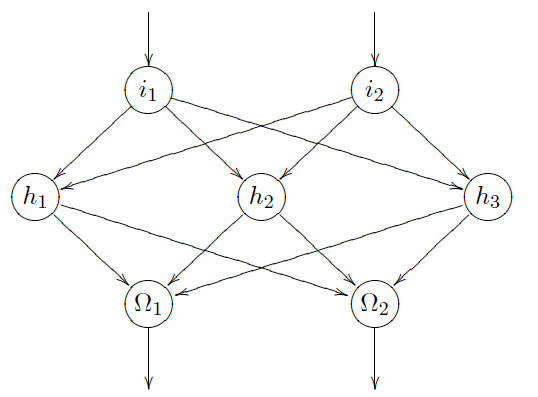
\includegraphics[width=\textwidth]{./img/Feedforward-normal-Topology.png}
	\caption{Standard feedforward topology}
	\end{subfigure}
	\begin{subfigure}[b]{0.3\textwidth}
	\centering
	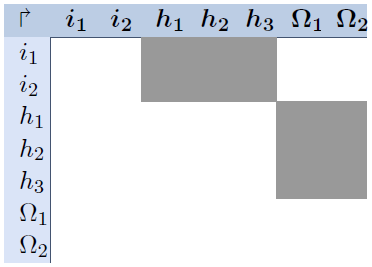
\includegraphics[width=\textwidth]{./img/Feedforward-normal-Hinton.png}
	\caption{Standard feedforward Hinton diagram}
	\end{subfigure}
\caption{Standard feedforward network; Source:\citep{Kriesel2013}}
\label{fig:feedforward}
\end{figure}
\paragraph{Shortcut connections.}
This is essentially a standard feedforward network (see ~\ref{par:feedforward}) where connections exist that skip one or more levels. these so-called shortcut connections may only be directed towards the output layer. (Figure ~\ref{fig:shortcutfeedforward})
\begin{definition}
(Shortcut feedforward). A shortcut feedforward network consists of three types of layers, one input layer, one output layer and optionally one or more processing layers. These layers are clearly separated. Connections only exist directed towards the output layer, the connections however may span over one or more layers.
\end{definition}
\begin{figure}
\centering
	\begin{subfigure}[b]{0.3\textwidth}
	\centering
	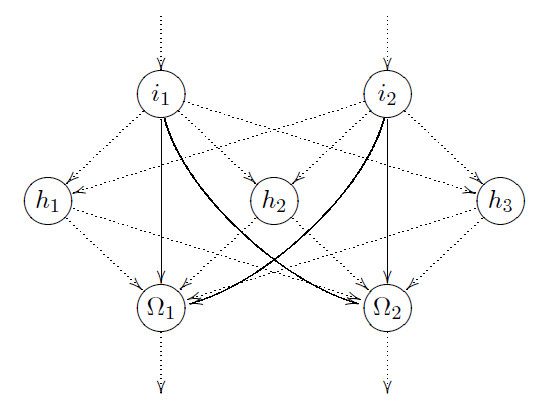
\includegraphics[width=\textwidth]{./img/Feedforward-shortcut-Topology.png}
	\caption{Shortcut feedforward topology}
	\end{subfigure}
	\begin{subfigure}[b]{0.3\textwidth}
	\centering
	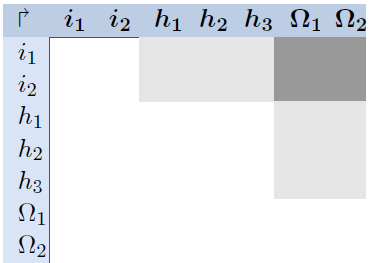
\includegraphics[width=\textwidth]{./img/Feedforward-shortcut-Hinton.png}
	\caption{Shortcut feedforward Hinton diagram}
	\end{subfigure}
\caption{Shortcut feedforward network; Source:\citep{Kriesel2013}}
\label{fig:shortcutfeedforward}
\end{figure}
\subsubsection{Recurrent networks}
Recurrence is the event where a neuron influences itself. This can be done through any means or by any connection. It is because of this that recurrent networks often don't have explicitly defined input and output neurons.
\paragraph{Direct recurrent.}
Direct recurrence happens in a network when neurons feed their output back to themselves as input. This is also often called self-recurrence. The neurons inhibit themselves, and as a result of this strengthen themselves in order to reach their activation limits. (Figure ~\ref{fig:directrecurrent})
\begin{definition}
(Direct recurrence). A direct recurrence network is a network where a neuron $j$ is connected to itself. the connection weight is then defined as $w_{j,j}$. The diagonal of weight matrix $W$ will no longer be zero as a direct result from this.
\end{definition}
\begin{figure}
\centering
	\begin{subfigure}[b]{0.3\textwidth}
	\centering
	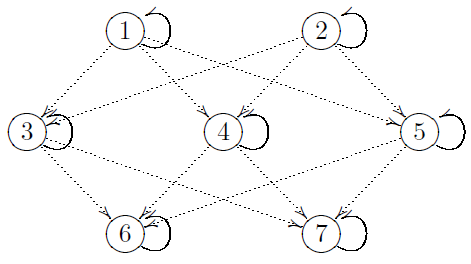
\includegraphics[width=\textwidth]{./img/recurrent-direct-Topology.png}
	\caption{Direct recurrent topology}
	\end{subfigure}
	\begin{subfigure}[b]{0.3\textwidth}
	\centering
	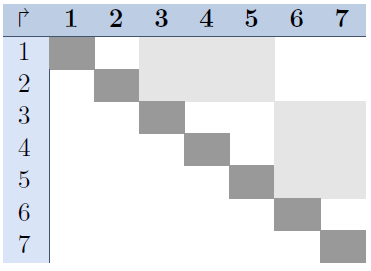
\includegraphics[width=\textwidth]{./img/recurrent-direct-Hinton.png}
	\caption{Direct recurrent Hinton diagram; Source:\citep{Kriesel2013}}
	\end{subfigure}
\caption{Direct recurrent network}
\label{fig:directrecurrent}
\end{figure}
\paragraph{Indirect recurrent.}
Indirect recurrence happens when in a network connections towards the input layer are allowed. A neuron can influence itself by passing its output to one of the previous or one of the next layers. (Figure ~\ref{fig:inderectrecurrence})
\begin{definition}
(Indirect recurrence). An indirect recurrent network is a network where connections forward and backward in the network may exist. The neurons influence themselves by influencing the preceding layers.
\end{definition}
\begin{figure}
\centering
	\begin{subfigure}[b]{0.3\textwidth}
	\centering
	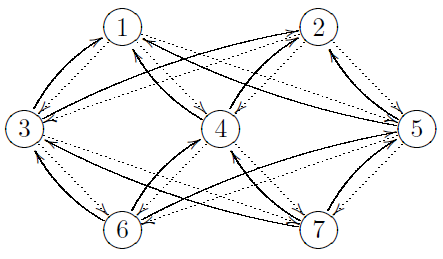
\includegraphics[width=\textwidth]{./img/recurrent-indirect-Topology.png}
	\caption{Indirect recurrent topology}
	\end{subfigure}
	\begin{subfigure}[b]{0.3\textwidth}
	\centering
	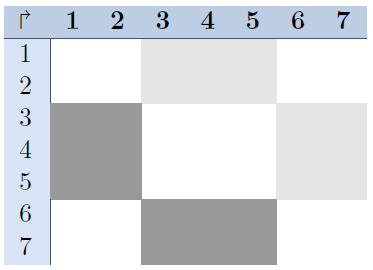
\includegraphics[width=\textwidth]{./img/recurrent-indirect-Hinton.png}
	\caption{Indirect recurrent Hinton diagram; Source:\citep{Kriesel2013}}
	\end{subfigure}
\caption{Indirect recurrent network}
\label{fig:inderectrecurrence}
\end{figure}
\paragraph{Lateral recurrent.}
Lateral recurrence happens when connections between neurons of the same layer exist. These connections often make it so that each neuron inhibits the other neurons and strengthens itself. This often means that only the strongest neuron becomes active (\emph{winner-takes-all scheme}). (Figure ~\ref{fig:lateralrecurrence})
\begin{definition}
(Lateral recurrence). A lateral recurrent network is a network where connections between the neurons of the same layer are allowed.
\end{definition}
\begin{figure}
\centering
	\begin{subfigure}[b]{0.3\textwidth}
	\centering
	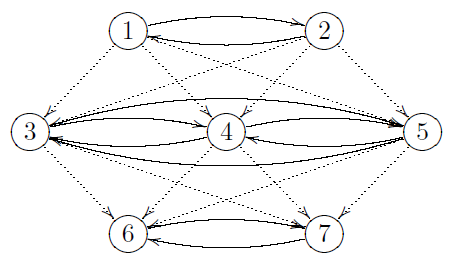
\includegraphics[width=\textwidth]{./img/recurrent-lateral-Topology.png}
	\caption{Lateral recurrent topology}
	\end{subfigure}
	\begin{subfigure}[b]{0.3\textwidth}
	\centering
	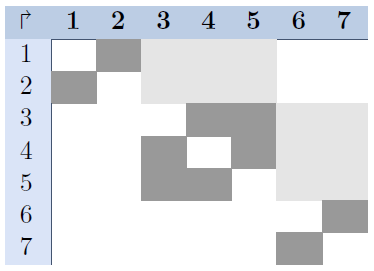
\includegraphics[width=\textwidth]{./img/recurrent-lateral-Hinton.png}
	\caption{Lateral recurrent Hinton diagram; Source:\citep{Kriesel2013}}
	\end{subfigure}
\caption{Lateral recurrent network}
\label{fig:lateralrecurrence}
\end{figure}
\subsubsection{Completely linked networks}
A completely linked network happens when all neuron connections are allowed, except for direct recurrent connections. All neuron connections must be symmetric, this means that $w_{i,j} = w_{j,i}$. As a direct result of the complete linking, input and output neurons can no longer be strictly defined and clearly defined layers do not longer exist. Another result is that the weight matrix $W$ can be different from zero everywhere, except along the diagonal. (Figure ~\ref{fig:completelylinked})
\begin{definition}
(Complete interconnection). A complete interconnected network is a network where each neuron is always connected to every other neuron. As a result ever neuron can become an input neuron.
\end{definition}
\begin{figure}
\centering
	\begin{subfigure}[b]{0.3\textwidth}
	\centering
	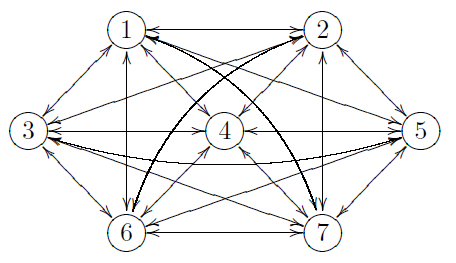
\includegraphics[width=\textwidth]{./img/Completelylinked-Topology.png}
	\caption{Completely linked topology}
	\end{subfigure}
	\begin{subfigure}[b]{0.3\textwidth}
	\centering
	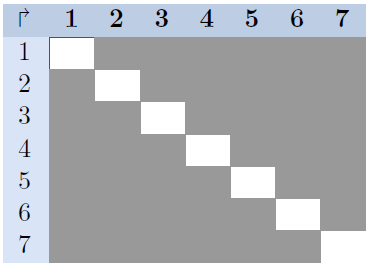
\includegraphics[width=\textwidth]{./img/Completelylinked-Hinton.png}
	\caption{Completely linked Hinton diagram; Source:\citep{Kriesel2013}}
	\end{subfigure}
\caption{Completely linked network}
\label{fig:completelylinked}
\end{figure}
\subsection{Neural network learning}
One of the most interesting features of a neural network is the ability to familiarize themselves with a problem by means of training. This means that after sufficient training, the network will be able to solve unknown problems of the same type. This is called generalization. Training a  network involves some form of leaning procedure. A learning procedure is a rather complex thing, so a brief explanation will be giving first.
\paragraph{Learning paradigms.}
We must be careful with the term ''learning'' as it is a very comprehensive term. A system learns when it changes itself in order to adapt to changes in the systems environment. A neural network as a learning systems changes, learns, whenever its components change. So any change in the components previously  mentioned due to environmental changes will result in a changing network. this process is classified as neural network learning. Looking ad the previous components capable of changing we can form a list of all theoretically possible means of neural network learning.
\begin{enumerate}
\item developing new connections
\item deleting existing connections
\item changing connecting weights
\item changing the threshold values of neurons
\item varying one or more of the three neuron functions (activation function, propagation function and output function)
\item developing new neurons
\item deleting existing neurons (and so its existing connections)
\end{enumerate}
We can safely assume that changing the connection weights will be the most commonly used method of training. Especially because of the simple fact that deleting a connection (no longer training a connection with weight) and creating new connections (changing the connection weight from 0) in the connection matrix can be done by connection weight adjustment training. With the introduction of the bias neuron (~\ref{subsubsec:biasneuron}) the threshold values can also be changed by using connection weight training.  We can perform any of the first four of the learning paradigms by just training synaptic weights.\\\\Changin neuron functions is difficult to implement and not very intuitive. Because of this, those paradigms aren't really popular and will not be discussed any further. The option of generating new, or removing old neurons have a few advantages. This method not only provides a way to keep the connection weights well adjusted during the training of a neural network, it also optimizes the neural network topology. For this reason this type of training is gathering a growing amount of interest. A method of achieving this functionality would be evolutionary algorithms. However we will not elaborate any further on this since this is outside the scope of this thesis, and since we already covered that the majority of learning methods can be achieved by weight training.\\\\To summarize, neural network learn by modifying the connecting weights according to rules formulated as algorithms. Therefore a learning procedure is always an algorithm that can easily be implemented by means of a programming language.
\paragraph{Training patterns, teaching input, desired output and error vector}
\begin{definition}
(Desired output). The expected result of the output layer when presented with a training pattern.
\end{definition}
\begin{definition}
(Teaching input). For an output neuron $j$ the teaching input $t_j$ is desired and correct value $j$ should have after the input of a training pattern. The teaching inputs $t_1,t_2, \dotsc ,t_n$ van be combined into a vector $t$. $t$ always refers to a specific training pattern $p$. this correlation is contained in the training set.
\end{definition}
\begin{definition}
(Training pattern). A training pattern is an input vector $p$ with the components $p_1,p_2, \dotsc , p_n$ whose desired output is known. By entering the training pattern into the network we receive an output that can be compared with the desired output. 
\end{definition}
\begin{definition}
(Training set). A training set (named $P$) is a finite set of pairs of training patterns ($p$) and teaching inputs ($t$). The finite ordered pairs $(p,t)$ of training patterns and teaching inputs are used to train our neural network.
\end{definition}
\begin{definition}
(Error vector).The error vector (also called the difference vector) for output neurons $\Omega_1,\Omega_2, \dotsc ,\Omega_n$ is the difference between the actual output vector and the teaching input for a training input $p$. Depending on whether you are learning offline or online, the difference vector refers to a specific training pattern, or to the error of a set of training patterns which is normalized in a certain way.\begin{center}
$E_p = 	\begin{pmatrix}
			t_1-y_1\\
			t_2-y_2\\
			\vdots\\
			t_n-y_n
		\end{pmatrix}$
\end{center}
\end{definition}
\subparagraph{Unsupervised learning.}
\subparagraph{Reinforced learning.}
\subparagraph{Supervised learning.}
\subparagraph{Offline learning.}
\paragraph{Training samples}
\paragraph{Learning curve and error measurement}
\paragraph{Hebbian rule}
\subsection{Supervised learning}
%TODO
TODO
\subsubsection{Preceptron networks}
%TODO
TODO
\subsubsection{Radial Basis networks}
%TODO
TODO
\subsubsection{Recurrent perceptron-like networks}
%TODO
TODO
\subsubsection{Hopfield networks}
%TODO
TODO
\subsubsection{Learning vector quantization}
%TODO
TODO
\subsection{Unsupervised learning}
%TODO
TODO
\subsubsection{Self-organizing maps}
%TODO
TODO
\subsubsection{Adaptive resonance theory}
%TODO
TODO
\subsubsection{Input and output of data}
%TODO
TODO
\section{Neural networks for pattern recognition}
sources and zever
%TODO
TODO
\subsection{Optimal network topologies}
%TODO
TODO
\subsubsection{Perceptron}
%TODO
TODO
\subsubsection{Hopfield}
%TODO
TODO
\subsubsection{Kohonen self organizing maps}
\subsection{Optimal network configuration}
%TODO
TODO
\section{Implementation}
\label{sec:implementation}
\subsection{Captcha builder}
%TODO
TODO
\subsection{Neural networks}
%TODO
TODO
\chapter{Conclusion}
\label{ch:conclusie}
%TODO
TODO
%
%%---------- Bijlagen ----------------------------------------------------
%
\appendix
%\chapter{Sourcecode}
%\label{ch:Sourcecode}
%
% Automatisch invoegen van al je Java broncode:
% 1/ maak een link naar je broncodedirectory naar subdirectory source
%      ln -s /path/to/java/src/ ./source
%    Of kopieer desnoods al je broncodebestanden. Zorg dat je
%    versiebeheersysteem deze directory negeert!
% 2/ Genereer source.tex met het script source.sh
%      ./source.sh
% 3/ Haal volgende regel uit commentaar
%% Java Broncode, gegenereerd door ./source.sh
% Waarschuwing: manuele wijzigingen worden overschreven!

\section{Package captchabuilder}

\section{Package captchacleanup}

\section{Package neuralnetworks}

\section{Package captchabuilder.builder}
\codefragment{source/captchabuilder/Captcha.java}{captchabuilder.Captcha}

\section{Package captchabuilder.elementcreator}

\section{Package captchabuilder.util}

\section{Package captchacleanup.image}

\section{Package captchacleanup.textfromimage}

\section{Package neuralnetworks.network}

\section{Package neuralnetworks.util}
\codefragment{source/captchabuilder/builder/BackgroundParser.java}{captchabuilder.builder.BackgroundParser}
\codefragment{source/captchabuilder/builder/BorderParser.java}{captchabuilder.builder.BorderParser}
\codefragment{source/captchabuilder/builder/CaptchaBuilder.java}{captchabuilder.builder.CaptchaBuilder}
\codefragment{source/captchabuilder/builder/CaptchaBuildSequenceParser.java}{captchabuilder.builder.CaptchaBuildSequenceParser}
\codefragment{source/captchabuilder/builder/ColorsParser.java}{captchabuilder.builder.ColorsParser}
\codefragment{source/captchabuilder/builder/GimpyParser.java}{captchabuilder.builder.GimpyParser}
\codefragment{source/captchabuilder/builder/NoiseParser.java}{captchabuilder.builder.NoiseParser}
\codefragment{source/captchabuilder/builder/TextParser.java}{captchabuilder.builder.TextParser}
\codefragment{source/captchabuilder/elementcreator/CaptchaElementCreatorBuilder.java}{captchabuilder.elementcreator.CaptchaElementCreatorBuilder}

\section{Package captchabuilder.elementcreator.producer}

\section{Package captchabuilder.elementcreator.renderer}
\codefragment{source/captchabuilder/util/ArrayUtil.java}{captchabuilder.util.ArrayUtil}
\codefragment{source/captchabuilder/util/CaptchaDAO.java}{captchabuilder.util.CaptchaDAO}
\codefragment{source/captchabuilder/util/ColorRangeRGBA.java}{captchabuilder.util.ColorRangeRGBA}

\section{Package captchabuilder.util.enums}
\codefragment{source/captchabuilder/util/ImageUtil.java}{captchabuilder.util.ImageUtil}
\codefragment{source/captchacleanup/image/ImageToArray.java}{captchacleanup.image.ImageToArray}
\codefragment{source/captchacleanup/image/ImageUtils.java}{captchacleanup.image.ImageUtils}
\codefragment{source/captchacleanup/textfromimage/GetImageText.java}{captchacleanup.textfromimage.GetImageText}
\codefragment{source/captchacleanup/textfromimage/TextRegion.java}{captchacleanup.textfromimage.TextRegion}

\section{Package neuralnetworks.network.encog}
\codefragment{source/neuralnetworks/network/NeuralNetworkActions.java}{neuralnetworks.network.NeuralNetworkActions}
\codefragment{source/neuralnetworks/network/NeuralNetwork.java}{neuralnetworks.network.NeuralNetwork}
\codefragment{source/neuralnetworks/util/CharacterPatternUtils.java}{neuralnetworks.util.CharacterPatternUtils}
\codefragment{source/neuralnetworks/util/EncogTrainingSet.java}{neuralnetworks.util.EncogTrainingSet}
\codefragment{source/neuralnetworks/util/ImageToInputPattern.java}{neuralnetworks.util.ImageToInputPattern}

\section{Package captchabuilder.elementcreator.producer.background}

\section{Package captchabuilder.elementcreator.producer.border}

\section{Package captchabuilder.elementcreator.producer.noise}

\section{Package captchabuilder.elementcreator.producer.text}

\section{Package captchabuilder.elementcreator.renderer.gimpy}

\section{Package captchabuilder.elementcreator.renderer.text}
\codefragment{source/captchabuilder/util/enums/CaptchaConstants.java}{captchabuilder.util.enums.CaptchaConstants}

\section{Package captchabuilder.util.enums.producer}

\section{Package captchabuilder.util.enums.renderer}
\codefragment{source/neuralnetworks/network/encog/EncogBasicNetworkBuilder.java}{neuralnetworks.network.encog.EncogBasicNetworkBuilder}
\codefragment{source/neuralnetworks/network/encog/EncogBasicNetwork.java}{neuralnetworks.network.encog.EncogBasicNetwork}
\codefragment{source/neuralnetworks/network/encog/EncogHopfieldNetworkBuilder.java}{neuralnetworks.network.encog.EncogHopfieldNetworkBuilder}
\codefragment{source/neuralnetworks/network/encog/EncogHopfieldNetwork.java}{neuralnetworks.network.encog.EncogHopfieldNetwork}

\section{Package neuralnetworks.network.encog.util}
\codefragment{source/captchabuilder/elementcreator/producer/background/AbstractBackgroundProducer.java}{captchabuilder.elementcreator.producer.background.AbstractBackgroundProducer}
\codefragment{source/captchabuilder/elementcreator/producer/background/BackgroundProducerBuilder.java}{captchabuilder.elementcreator.producer.background.BackgroundProducerBuilder}
\codefragment{source/captchabuilder/elementcreator/producer/background/BackgroundProducer.java}{captchabuilder.elementcreator.producer.background.BackgroundProducer}
\codefragment{source/captchabuilder/elementcreator/producer/background/FlatColorBackgroundProducer.java}{captchabuilder.elementcreator.producer.background.FlatColorBackgroundProducer}
\codefragment{source/captchabuilder/elementcreator/producer/background/SquigglesBackgroundProducer.java}{captchabuilder.elementcreator.producer.background.SquigglesBackgroundProducer}
\codefragment{source/captchabuilder/elementcreator/producer/background/TransparentBackgroundProducer.java}{captchabuilder.elementcreator.producer.background.TransparentBackgroundProducer}
\codefragment{source/captchabuilder/elementcreator/producer/background/TwoColorGradientBackgroundProducer.java}{captchabuilder.elementcreator.producer.background.TwoColorGradientBackgroundProducer}
\codefragment{source/captchabuilder/elementcreator/producer/border/AbstractBorderProducer.java}{captchabuilder.elementcreator.producer.border.AbstractBorderProducer}
\codefragment{source/captchabuilder/elementcreator/producer/border/BorderProducerBuilder.java}{captchabuilder.elementcreator.producer.border.BorderProducerBuilder}
\codefragment{source/captchabuilder/elementcreator/producer/border/BorderProducer.java}{captchabuilder.elementcreator.producer.border.BorderProducer}
\codefragment{source/captchabuilder/elementcreator/producer/border/SolidBorderProducer.java}{captchabuilder.elementcreator.producer.border.SolidBorderProducer}
\codefragment{source/captchabuilder/elementcreator/producer/noise/AbstractNoiseProducer.java}{captchabuilder.elementcreator.producer.noise.AbstractNoiseProducer}
\codefragment{source/captchabuilder/elementcreator/producer/noise/CurvedLineNoiseProducer.java}{captchabuilder.elementcreator.producer.noise.CurvedLineNoiseProducer}
\codefragment{source/captchabuilder/elementcreator/producer/noise/NoiseProducerBuilder.java}{captchabuilder.elementcreator.producer.noise.NoiseProducerBuilder}
\codefragment{source/captchabuilder/elementcreator/producer/noise/NoiseProducer.java}{captchabuilder.elementcreator.producer.noise.NoiseProducer}
\codefragment{source/captchabuilder/elementcreator/producer/noise/StraightLineNoiseProducer.java}{captchabuilder.elementcreator.producer.noise.StraightLineNoiseProducer}
\codefragment{source/captchabuilder/elementcreator/producer/text/AbstractTextProducer.java}{captchabuilder.elementcreator.producer.text.AbstractTextProducer}
\codefragment{source/captchabuilder/elementcreator/producer/text/AlphanumericTextProducer.java}{captchabuilder.elementcreator.producer.text.AlphanumericTextProducer}
\codefragment{source/captchabuilder/elementcreator/producer/text/ArabicTextProducer.java}{captchabuilder.elementcreator.producer.text.ArabicTextProducer}
\codefragment{source/captchabuilder/elementcreator/producer/text/ChineseTextProducer.java}{captchabuilder.elementcreator.producer.text.ChineseTextProducer}
\codefragment{source/captchabuilder/elementcreator/producer/text/LetterTextProducer.java}{captchabuilder.elementcreator.producer.text.LetterTextProducer}
\codefragment{source/captchabuilder/elementcreator/producer/text/NumbersProducer.java}{captchabuilder.elementcreator.producer.text.NumbersProducer}
\codefragment{source/captchabuilder/elementcreator/producer/text/ReducedAlphanumericTextProducer.java}{captchabuilder.elementcreator.producer.text.ReducedAlphanumericTextProducer}
\codefragment{source/captchabuilder/elementcreator/producer/text/SpecialAlphanumericTextProducer.java}{captchabuilder.elementcreator.producer.text.SpecialAlphanumericTextProducer}
\codefragment{source/captchabuilder/elementcreator/producer/text/SpecialLetterTextProducer.java}{captchabuilder.elementcreator.producer.text.SpecialLetterTextProducer}
\codefragment{source/captchabuilder/elementcreator/producer/text/SpecialNumbersProducer.java}{captchabuilder.elementcreator.producer.text.SpecialNumbersProducer}
\codefragment{source/captchabuilder/elementcreator/producer/text/TextProducerBuilder.java}{captchabuilder.elementcreator.producer.text.TextProducerBuilder}
\codefragment{source/captchabuilder/elementcreator/producer/text/TextProducer.java}{captchabuilder.elementcreator.producer.text.TextProducer}
\codefragment{source/captchabuilder/elementcreator/renderer/gimpy/AbstractGimpyRenderer.java}{captchabuilder.elementcreator.renderer.gimpy.AbstractGimpyRenderer}
\codefragment{source/captchabuilder/elementcreator/renderer/gimpy/BlockGimpyRenderer.java}{captchabuilder.elementcreator.renderer.gimpy.BlockGimpyRenderer}
\codefragment{source/captchabuilder/elementcreator/renderer/gimpy/DropShadowGimpyRenderer.java}{captchabuilder.elementcreator.renderer.gimpy.DropShadowGimpyRenderer}
\codefragment{source/captchabuilder/elementcreator/renderer/gimpy/FishEyeGimpyRenderer.java}{captchabuilder.elementcreator.renderer.gimpy.FishEyeGimpyRenderer}
\codefragment{source/captchabuilder/elementcreator/renderer/gimpy/GimpyRendererBuilder.java}{captchabuilder.elementcreator.renderer.gimpy.GimpyRendererBuilder}
\codefragment{source/captchabuilder/elementcreator/renderer/gimpy/GimpyRenderer.java}{captchabuilder.elementcreator.renderer.gimpy.GimpyRenderer}
\codefragment{source/captchabuilder/elementcreator/renderer/gimpy/RippleGimpyRenderer.java}{captchabuilder.elementcreator.renderer.gimpy.RippleGimpyRenderer}
\codefragment{source/captchabuilder/elementcreator/renderer/gimpy/ShearGimpyRenderer.java}{captchabuilder.elementcreator.renderer.gimpy.ShearGimpyRenderer}
\codefragment{source/captchabuilder/elementcreator/renderer/gimpy/StretchGimpyRenderer.java}{captchabuilder.elementcreator.renderer.gimpy.StretchGimpyRenderer}
\codefragment{source/captchabuilder/elementcreator/renderer/text/AbstractWordRenderer.java}{captchabuilder.elementcreator.renderer.text.AbstractWordRenderer}
\codefragment{source/captchabuilder/elementcreator/renderer/text/ColoredEdgesWordRenderer.java}{captchabuilder.elementcreator.renderer.text.ColoredEdgesWordRenderer}
\codefragment{source/captchabuilder/elementcreator/renderer/text/DefaultWordRenderer.java}{captchabuilder.elementcreator.renderer.text.DefaultWordRenderer}
\codefragment{source/captchabuilder/elementcreator/renderer/text/WordRendererBuilder.java}{captchabuilder.elementcreator.renderer.text.WordRendererBuilder}
\codefragment{source/captchabuilder/elementcreator/renderer/text/WordRenderer.java}{captchabuilder.elementcreator.renderer.text.WordRenderer}
\codefragment{source/captchabuilder/util/enums/producer/BackgroundProducerType.java}{captchabuilder.util.enums.producer.BackgroundProducerType}
\codefragment{source/captchabuilder/util/enums/producer/BorderProducerType.java}{captchabuilder.util.enums.producer.BorderProducerType}
\codefragment{source/captchabuilder/util/enums/producer/NoiseProducerType.java}{captchabuilder.util.enums.producer.NoiseProducerType}
\codefragment{source/captchabuilder/util/enums/producer/TextProducerType.java}{captchabuilder.util.enums.producer.TextProducerType}
\codefragment{source/captchabuilder/util/enums/renderer/GimpyRendererType.java}{captchabuilder.util.enums.renderer.GimpyRendererType}
\codefragment{source/captchabuilder/util/enums/renderer/WordRendererType.java}{captchabuilder.util.enums.renderer.WordRendererType}
\codefragment{source/neuralnetworks/network/encog/util/PropagationType.java}{neuralnetworks.network.encog.util.PropagationType}

%
\bibliographystyle{plainnat}
\bibliography{Solving_CAPTCHA_using_neural_networks}
%
%%---------- Back matter -------------------------------------------------
%
\listoffigures
\begin{figure}
	\centering
	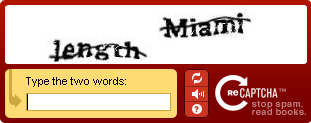
\includegraphics[width=\textwidth]{./img/reCAPTCHA.png}
	\caption{The reCAPTCHA system (Source: \citep{UNDP2013})}
	\label{fig:reCAPTCHA}
\end{figure}
\begin{figure}
\centering
	\begin{subfigure}[b]{0.5\textwidth}
		\centering
		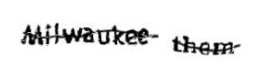
\includegraphics[width=\textwidth]{./img/reCAPTCHA2008.png}
		\caption{Early 2008}
	\end{subfigure}
	\begin{subfigure}[b]{0.5\textwidth}
		\centering
		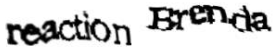
\includegraphics[width=\textwidth]{./img/reCAPTCHA2009.png}
		\caption{December 16th 2009}
	\end{subfigure}
	\begin{subfigure}[b]{0.5\textwidth}
		\centering
		
\includegraphics[width=\textwidth]{./img/reCAPTCHA2010.png}
		\caption{January 24th 2010}
	\end{subfigure}
	\begin{subfigure}[b]{0.5\textwidth}
		\centering
		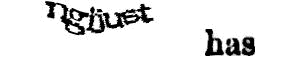
\includegraphics[width=\textwidth]{./img/reCAPTCHA2013.png}
		\caption{May 28th 2013}
	\end{subfigure}
	\caption{Examples of CAPTCHAs directly Downloaded from reCAPTCHA (Source: \citep{Motoyama2010} and \citep{reCAPTCHA2013})}
	\label{fig:captchaEvolution}
\end{figure}
\begin{figure}
\centering
	\begin{subfigure}[b]{0.65\textwidth}
		\centering
		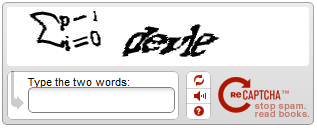
\includegraphics[width=\textwidth]{./img/impossible_captcha01.png}
		\caption{Impossible CAPTCHA (Source: \url{http://asmallpieceofgodsplan.blogspot.be/2012/04/captchas.html} Accessed on 2013-0528)}
	\end{subfigure}
	\begin{subfigure}[b]{0.65\textwidth}
		\centering
		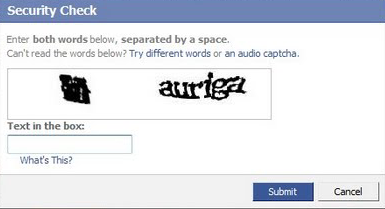
\includegraphics[width=\textwidth]{./img/impossible_captcha02.png}
		\caption{Impossible CAPTCHA (Source: \url{http://asmallpieceofgodsplan.blogspot.be/2012/04/captchas.html} Accessed on 2013-0528)}
	\end{subfigure}
	\begin{subfigure}[b]{0.65\textwidth}
		\centering
		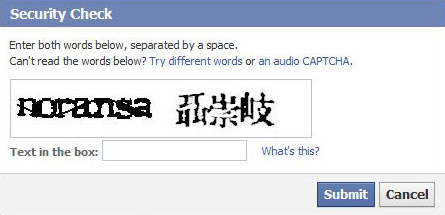
\includegraphics[width=\textwidth]{./img/impossible_captcha03.png}
		\caption{Impossible CAPTCHA (Source: \url{http://oactechnology.com/it-blog/blog/2012/08/31/captcha/} Accessed on 2013-0528)}
	\end{subfigure}
	\begin{subfigure}[b]{0.65\textwidth}
		\centering
		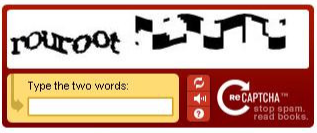
\includegraphics[width=\textwidth]{./img/impossible_captcha04.png}
		\caption{Impossible CAPTCHA (Source: \url{http://ragegenerator.com/pages/comic/39222} Accessed on 2013-0528)}
	\end{subfigure}
	\caption{Examples of CAPTCHAs nearly impossible to solve}
	\label{fig:ImpossibleCaptcha}
\end{figure}
\begin{figure}
	\centering
	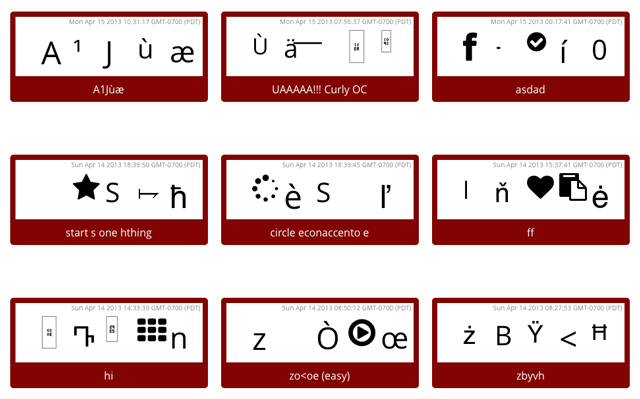
\includegraphics[width=\textwidth]{./img/CRAPCHA.png}
	\caption{Test generated by the CAPTCHA system (Source: \citep{Lsquid2013})}
	\label{fig:CRAPCHA}
\end{figure}
\begin{figure}
	\centering
	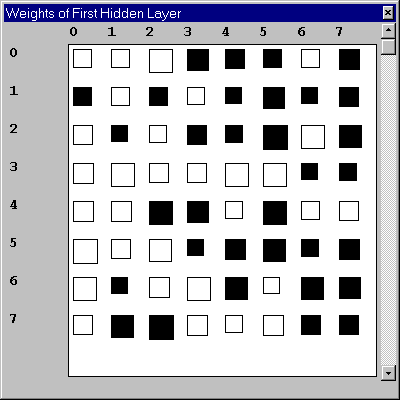
\includegraphics[width=\textwidth]{./img/Hinton_Diagram.png}
	\caption{An example Hinton diagram (Source: \url{http://www.nd.com/products/nsv30/hinton.htm})}
	\label{fig:HintonDiagram}
\end{figure}
%\listoftables
%
% Lijst van broncode-listings. Kan je weglaten als je dit niet nodig hebt.
%\lstlistoflistings
%
\end{document}